\documentclass[hyperref=unicode]{beamer}

\usepackage[absolute,overlay]{textpos}
\usepackage{graphicx}
\usepackage{adjustbox}
\usepackage{mhchem}
\usepackage{wrapfig}
\usepackage{ucs}
\usepackage[utf8]{inputenc}
\PrerenderUnicode{ěščřžýáíéĚŠČŘŽÝÁÍÉďťňĎŤŇůúÚóÓ}

\usepackage{tikz}
\usetikzlibrary{positioning}
\usetikzlibrary{arrows}
\usetikzlibrary{shapes.multipart}

\adjustboxset*{center}

\usepackage[czech]{babel}
\mode<presentation>{\usetheme{default}}
\DefineNamedColor{named}{pozadi}{RGB}{200,200,200}
\usecolortheme{crane}

\setbeamertemplate{footline}[frame number]

\addtobeamertemplate{frametitle}{
   \let\insertframetitle\insertsectionhead}{}
\addtobeamertemplate{frametitle}{
   \let\insertframesubtitle\insertsubsectionhead}{}

\makeatletter
  \CheckCommand*\beamer@checkframetitle{\@ifnextchar\bgroup\beamer@inlineframetitle{}}
  \renewcommand*\beamer@checkframetitle{\global\let\beamer@frametitle\relax\@ifnextchar\bgroup\beamer@inlineframetitle{}}
\makeatother
\setbeamercolor{section in toc}{fg=blue}
\setbeamertemplate{section in toc shaded}[default][100]

\begin{document}
\title[Crisis]
{Infračervená a Ramanova spektroskopie}

\author
{Zdeněk Moravec}
\date[KPT 2004]
{hugo@chemi.muni.cz}

\frame{\titlepage}

\section{Osnova}
\frame{
	\frametitle{}
	\vfill
	\begin{itemize}
	\item Základní principy IR spektroskopie
	\item Měřící techniky
	\begin{itemize}
		\item FT-IR transmisní měření
		\item ATR, DRIFT, PAS
		\item TG/IR, GC/IR
	\end{itemize}
	\item Ramanova spektroskopie
	\item Zpracování spekter
	\begin{itemize}
		\item Analýza spekter
		\item Spektrální databáze
	\end{itemize}
	\item Aplikace
	\begin{itemize}
		\item Chemie
		\item Restaurování uměleckých předmětů
		\item Biologie
	\end{itemize}
	\item Informace o přístrojovém vybavení UCH
	\end{itemize}
	\vfill
}

\section{Molekulová spektroskopie}
\frame{
	\frametitle{}
	\vfill
	\begin{tabular}{|p{2.2cm}|p{3cm}|p{2cm}|p{2cm}|}
	\hline
	& UV-VIS & IR & MW \\
	& 50-800 nm & 1-100 $\mu$m & 1-10 mm \\
	\hline
	Elektronická
	\newline spektroskopie & Absorpční UV-VIS 
	\newline Luminiscenční spektroskopie & & \\
	\hline
	Vibrační 
	\newline spektroskopie & Ramanova spektroskopie & Infračervená spektroskopie & \\
	\hline
	Rotační 
	\newline spektroskopie & Ramanova spektroskopie & & Mikrovlnná spektroskopie \\
	\hline
	\end{tabular}
	\vfill
}

\section{IR spektroskopie}
\subsection{Princip}
\frame{
	\frametitle{}
	\vfill
	\adjincludegraphics[width=250pt,valign=t]{img/em-spectrum.png}
	\vfill
}

\frame{
	\frametitle{}
	\vfill
	\adjincludegraphics[width=250pt,valign=t]{img/el-prechody.png}
	\vfill
}

\frame{
	\frametitle{}
	\vfill
	\begin{itemize}
	\item  NIR (0,7 -- 2,5 $\mu$m; 14 000 - 4 000 cm$^{-1}$) - infračervená spektroskopie v blízké oblasti
	\item  MIR (2,5 -- 25 $\mu$m; 4 000 - 400 cm$^{-1}$) - infračervená spektroskopie ve střední oblasti
	\item  FIR (25 -- 1000 $\mu$m; 400 - 10 cm$^{-1}$) - infračervená spektroskopie ve vzdálené oblasti
	\end{itemize}
	\vfill
}

\subsection{Vibrace chemických vazeb}
\frame{
	\frametitle{}
	\vfill
	\begin{itemize}
	\item Během vibrace vazby dochází k přechodu systému na jinou energetickou hladinu.
	\item Přechod mezi základní a 1. excitovanou hladinou se nazývá \em základní (fundamentální) vibrace \em.
	\item Pokud dochází k přechodům na vyšší hladinu, jedná se o tzv. \em vyšší harmonické přechody (overtony) \em. Jejich frekvence jsou \em přibližně \em násobkem fundamentální frekvence (energetické hladiny se postupně zhušťují).
	\item Pokud dojde k současné změně dvou vibračních stav molekuly jedná se o \em kombinační přechody \em.

	\end{itemize}
	\vfill
}

\frame{
	\frametitle{}
	\vfill
	\begin{itemize}
	\item Valenční vibrace – dochází ke změně mezijaderné vzdálenosti.
	\item Deformační vibrace – dochází ke změně vazebného úhlu.
	\end{itemize}
	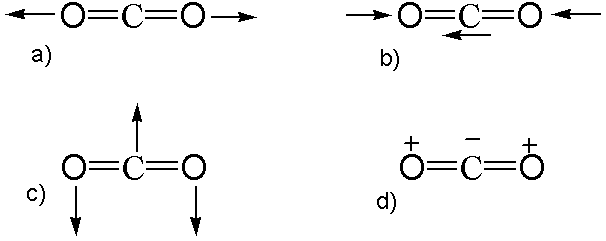
\includegraphics[scale=0.4]{img/CO2-vibration.png}
	\vfill
}


\subsection{Dipólový moment}
\frame{
	\frametitle{}
	\vfill
	\begin{itemize}
	\item Vektor popisující rozložení elektrického náboje v molekule.
	\item Výsledný dipólmoment získáme vektorovým součtem dipólmomentů jednotlivých vazeb.
	\end{itemize}
\begin{columns}
\column{0.6\textwidth}
\begin{center}
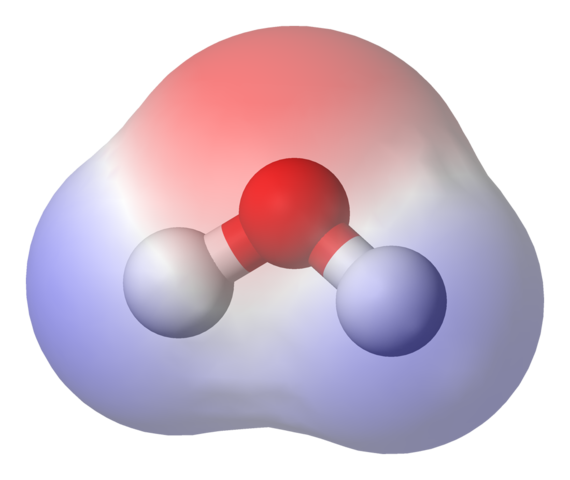
\includegraphics[width=5cm]{img/water-elpot.png}
\end{center}

\column{0.4\textwidth}
\begin{center}
\begin{picture}(0,0)
\put(0,0){O}
\put(23,-30){H}
\put(-23,-30){H}
\thicklines
\put(4,-1){\vector(-1,-1){20}}
\put(4,-1){\vector(1,-1){20}}
\put(4,-1){\vector(0,-1){40}}
\thinlines
\put(24,-21){\line(-1,-1){20}}
\put(-16,-21){\line(1,-1){20}}
\end{picture}
\end{center}
\end{columns}
	\vfill
}

\section{Absorpce infračerveného záření}
\frame{
	\frametitle{}
	\vfill
	\begin{itemize}
	\item Aby mohla molekula absorbovat infračervené záření musí během vibrace docházet ke změně dipólového momentu.
	\item Při absorpci dochází ke změně amplitudy vibrace, frekvence zůstává nezměněna.
	\item Intenzita absorpčních pásu je úměrná druhé mocnině změny dipólového momentu.
	\item Absorpcí infračerveného záření molekulami vznikají pásová spektra.
	\end{itemize}
	\vfill
}

\subsection{Absorpční spektrum}
\frame{
	\frametitle{}
	\vfill
	\adjincludegraphics[width=300pt,valign=l]{img/spectrum.png}
	\begin{textblock*}{1cm}[1,1](55mm,65mm)
	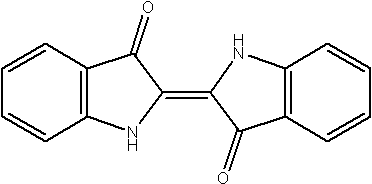
\includegraphics[width=80pt]{img/spectrum-struct.png}
	\end{textblock*}
	\begin{itemize}
	\item Absorpční spektrum indiga
	\end{itemize}
	\vfill
}

\section{Měřící techniky}
\frame{
	\frametitle{}
	\vfill
	\begin{itemize}
	\item  FT-IR - transmise, ATR
	\item  DRIFT, IRRAS
	\item TG-IR, GC-IR
	\end{itemize}
	\vfill
}

\subsection{FT-IR}
\frame{
	\frametitle{}
	\vfill
	\begin{itemize}
	\item  Nejběžnější měřící technika
	\item Podle úpravy vzorku rozlišujeme měření v transmisním módu a ATR
	\item Spektrometr neobsahuje monochromátor, ale interferometr
	\item Celé spektrum se snímá najednou, získáme interferogram, který je nutné zpracovat pomocí Fourierovy transformace
	\end{itemize}
	\vfill
}

\frame{
	\frametitle{}
	\vfill
	\adjincludegraphics[width=11cm,valign=l]{img/ftir.png}
	\vfill
}

\subsection{Transmisní měření}
\frame{
	\frametitle{}
	\vfill
	\begin{itemize}
	\item  Lze měřit pevné látky, kapaliny i plyny
	\item Pevné látky měříme ve formě KBr tablet (1-3 hm. \% v KBr) nebo jako suspenze v Nujolu
	\item Kapaliny měříme jako tenký film mezi okny z vhodného materiálu (KBr, KRS, NaCl, ...)
	\end{itemize}
	\adjincludegraphics[width=300pt,valign=l]{img/kbr-pellets.png}
	\vfill
}

\subsection{Transmisní měření - Nujol}
\frame{
	\frametitle{}
	\vfill
	\begin{itemize}
	\item Nujol - směs alkanů s dlouhý řetězcem.
	\end{itemize}
	\adjincludegraphics[width=300pt,valign=l]{img/nujol.png}
	\vfill
}

\subsection{Transmisní měření plynů}
\frame{
	\frametitle{}
	\vfill
	\begin{itemize}
	\item Plyny se měří v plynových kyvetách, ty jsou konstruované tak, aby dráha paprsku byla co nejdelší
	\item Protože v plynném skupenství existují pouze slabé interakce mezi částicemi lze naměřit čistě rotační, rotačně-vibrační i elektronově-rotačně-vibrační spektra
	\end{itemize}
	\adjincludegraphics[width=90mm,valign=l]{img/water.png}
	\vfill
}

\subsection{ATR}
\frame{
	\frametitle{}
	\vfill
	\begin{itemize}
	\item ATR - Attenuated Total Reflection
	\item Krystaly jsou z diamantu, ZnSe, Ge, KRS-5 (směs TlBr a TlI) nebo křemíku
	\item Vzorek se přitlačí vysokým tlakem k měřícímu krystalu
	\item Paprsek se pohybuje po povrchu vzorku (0,5 - 5 $\mu$m)
	\end{itemize}
	\vfill
	\adjincludegraphics[width=180pt,valign=b]{img/atr.png}
}

\subsection{IRRAS}
\frame{
	\frametitle{}
	\vfill
	\begin{itemize}
	\item IRRAS - IR Reflection Absorption Spectroscopy
	\item Metoda vhodná pro tenké vrstvy nanesené na kovových materiálech nebo nasorbované látky na materiálech
	\item Pro zvýšení citlivosti se využívá polarizovaného záření
	\end{itemize}
	\adjincludegraphics[width=200pt,valign=l]{img/irras.png}
	\vfill
}

\subsection{DRIFTS}
\frame{
	\frametitle{}
	\vfill
	\begin{itemize}
	\item DRIFTS - Diffuse Reflectance Infrared Fourier Transform Spectroscopy
	\item Tato technika je vhodná pro měření malých částic nebo hrubých povrchů
	\item Využívá rozptylu IR záření
	\item Rozptýlené záření je pomocí kulového zrcadla odráženo na detektor
	\item Práškové vzorky se měří v kelímcích, pevné vzorky se obrousí abrasivem (SiC) a měří se částice zachycené na abrasivu
	\end{itemize}
	\adjincludegraphics[width=52mm,valign=l]{img/drifts.png}
	\vfill
}

\section{Coupling TGA/IR}
\frame{
	\frametitle{}
	\vfill
	\begin{itemize}
	\item TGA - termogravimetrická analýza
	\item Plyny vznikající během degradace vzorku vedeme do měřící cely a pomocí IR spektroskopie stanovíme jejich složení
	\item Během transportu plynů z pece do měřící cely dochází k velkému zředění plynu, proto je nutné používat citlivější detektory (MCT)
	\end{itemize}
	\adjincludegraphics[width=10cm,valign=l]{img/tg-irFoto.jpg}
	\vfill
}

\frame{
	\frametitle{}
	\vfill
	\adjincludegraphics[width=11cm,valign=l]{img/tg-ir.png}
	\vfill
}

\section{Coupling GC/IR}
\frame{
	\frametitle{}
	\vfill
	\begin{itemize}
	\item GC - plynová chromatografie
	\item Méně citlivé než GC/MS, ale umožňuje analýzu stereoizomerů.
	\item Interferogramy je nutné snímat v krátkých časových intervalech
	\end{itemize}
	\adjincludegraphics[width=10cm,valign=l]{img/gc-ir.jpg}
	\vfill
}

\section{Ramanova spektroskopie}
\subsection{Princip}
\frame{
	\frametitle{}
	\begin{itemize}
	\item Komplementární metoda k infračervené spektroskopii.
	\item 1928 – Sir Chandrasekhara Venkata Rāman objevil nepružný 
rozptyl záření (Ramanův rozptyl). 
	\item Využívá silné zdroje monochromatického záření – lasery.
	\item Při interakci se vzorkem dochází z největší části k Rayleighovu rozptylu, energie rozptýleného záření je stejná jako energie 
excitujícího záření.
	\item S nižší pravděpodobností dochází k Ramanovu rozptylu, kdy záření část své energie předává vzorku (Stokesovy linie) nebo ji naopak vzorku odebírá (Anti-Stokesovy linie).
	\item Aby mohlo dojít k Ramanovu rozptylu, děj musí být spojen se změnou tenzoru polarizovatelnosti.
	\end{itemize}
}


\frame{
	\frametitle{Polarizovatelnost}
	\vfill
	\begin{columns}
	\begin{column}{0.88\textwidth}
	\begin{itemize}
	\item Polarizovatelnost ($\alpha$) popisuje deformovatelnost elektronové hustoty v okolí molekuly působením elektromagnetického záření, nebo přesněji elektrického pole generovaného fotonem.
	\item Polarizovatelnost je \emph{tensor druhého řádu}, tzn. že ji lze popsat maticí $3\times3$.
	\item Polarizace je ovlivněna několika faktory:
	\begin{itemize}
		\item Čím více elektronů má atom, tím slaběji je k sobě váže a tím je polarizovatelnost větší.
		\item Čím je elektron více vzdálen od kladného jádra, tím je pohyblivější a zvyšuje polarizovatelnost atomu.
		\item Orientací molekuly vůči vnějšímu elektrickému poli.
	\end{itemize}
	\end{itemize}
	\end{column}
	\begin{column}{0.20\textwidth}
	\adjincludegraphics[width=30mm]{img/tensor-comp.png}
\scalebox{0.6}{
$
\alpha =
\begin{bmatrix}
\alpha_{xx} & \alpha_{xy} & \alpha_{xz}\\
\alpha_{yx} & \alpha_{yy} & \alpha_{yz}\\
\alpha_{zx} & \alpha_{zy} & \alpha_{zz}\\
\end{bmatrix}
$
}
	\end{column}
	\end{columns}
	\footnotetext[1]{\url{https://en.wikipedia.org/wiki/Polarizability}}
	\footnotetext[2]{\url{http://chemwiki.ucdavis.edu/Physical_Chemistry/Physical_Properties_of_Matter/Intermolecular_Forces/Polarizability}}
	\footnotetext[3]{\href{http://photonicswiki.org/index.php?title=Polarization_and_Polarizability}{Animace - polarizovatelnost}}
	\vfill
}

\frame{
	\frametitle{}
	\adjincludegraphics[width=12cm,valign=l]{img/RamanScattering.pdf}
	
	http://commons.wikimedia.org/wiki/File:Ramanscattering.svg
}

\frame{
	\frametitle{}
\begin{tikzpicture}
\node at (9,10.2) {LASER};
\draw [fill=black] (10,10) rectangle (8,9.5);
\draw [thick,->] (10,9.75) -- (12,9.75);

\draw [thick,<-] (8,9.3) -- (8,6.5);
\node at (7.9,9) {I};
\draw [thick,->] (8,6.5) -- (11.5,6.5);
\node at (11.3,6.3) {f};
\draw (8.3,6.8) -- (9.9,6.8);
\draw (10,6.8) -- (11.3,6.8);
\draw (9.9,6.8) -- (9.95,9);
\draw (10,6.8) -- (9.95,9);


\draw [fill=red,red] (12,11) rectangle (13,9);
\node [red] at (12.5,11.2) {Vzorek};
\draw [thick,->,red] (12.5,9) -- (12.5,7);
\draw [thick,->,red] (12.5,9) -- (13.5,7);
\draw [thick,->,red] (12.5,9) -- (11.5,7);
\draw [thick,->,red] (12.5,9) -- (13.0,7);
\draw [thick,->,red] (12.5,9) -- (12,7);

\draw [thick,blue] (12.0,6.5) arc [radius=0.5, start angle=180, end angle=360];
\draw [blue,fill=blue] (12.5,6.4) circle [radius=0.2];
\draw [thick,->,blue] (13.2,6.3) -- (14.5,6.3);
\node [blue] at (12.5,5.8) {Detektor};

\draw [thick,<-] (15.0,9.3) -- (15.0,6.0);
\node at (14.9,9.0) {I};
\draw [thick,->] (15.0,6.0) -- (19,6.0);
\node at (18.9,5.75) {$\tilde\nu$};

\draw (17.15,6.1) -- (17.2,9.3);
\draw (17.3,6.1) -- (17.25,9.3);

\draw (16.5,6.1) -- (16.54,6.6);
\draw (16.58,6.1) -- (16.54,6.6);

\draw (16.0,6.1) -- (16.02,7.4);
\draw (16.04,6.1) -- (16.02,7.4);

\draw (15.3,6.1) -- (15.33,7.0);
\draw (15.36,6.1) -- (15.33,7.0);

\draw (17.85,6.1) -- (17.89,6.3);
\draw (17.93,6.1) -- (17.89,6.3);

\draw (18.35,6.1) -- (18.37,6.9);
\draw (18.39,6.1) -- (18.37,6.9);

\draw (15.2,6.1) -- (15.3,6.1);
\draw (15.36,6.1) -- (16.0,6.1);
\draw (16.04,6.1) -- (16.5,6.1);
\draw (16.58,6.1) -- (17.15,6.1);
\draw (17.3,6.1) -- (17.85,6.1);
\draw (17.93,6.1) -- (18.35,6.1);
\draw (18.39,6.1) -- (18.8,6.1);

\node at (17.2,9.5) {Rayleigh};

\end{tikzpicture}
}

\subsection{Lasery}
\frame{
	\frametitle{}
	\adjincludegraphics[width=3cm,valign=l]{img/laser.png}
	\begin{itemize}
	\item Light Amplification by Stimulated Emission of Radiation
	\item He-Ne laser – 632,8 nm
	\item Ar laser – 488 nm, 496,5 nm a 514,4 nm
	\item Kr laser – 530,9 nm a 674,1 nm
	\item Nd:YAG laser – 1064 nm
	\item laserové diody
	\item laditelné lasery
	\end{itemize}
}

\subsection{Instrumentace}
\frame{
	\frametitle{}

	\begin{columns}
	\column{.5\textwidth}
	\adjincludegraphics[height=6cm,valign=l]{img/RamanPohled.jpg}
	
	\column{.5\textwidth}
	\adjincludegraphics[height=6cm,valign=l]{img/RamanVnitrek.jpg}
	\end{columns}
}

\frame{
	\frametitle{}
	\adjincludegraphics[width=11cm,valign=l]{img/FRA106.png}
}

\subsection{Příprava vzorku}
\frame{
	\frametitle{}
	\begin{itemize}
	\item Jednodušší než u IR spektroskopie.
	\item Pevné vzorky se měří ve skleněných kapilárách nebo jako tenké vrstvy na vhodném substrátu. Větší vzorky lze uchytit do držáku vzorku bez úpravy.
	\item Kapalné vzorky se také plní do kapilár.
	\item Pro měření plynných vzorků se využívají kyvety s násobným odrazem.
	\item Komplikací při měření bývá luminiscence vzorku. Lze ji potlačit změnou vlnové délky laseru, pokud to spektrometr umožňuje.
	\end{itemize}
}


\frame{
	\frametitle{}
	\adjincludegraphics[width=11cm,valign=l]{img/RamanSpectra.png}
}

\frame{
	\frametitle{Ramanova spektroskopie}
	\adjincludegraphics[width=10cm,valign=l]{img/Cappilaries.jpg}
}

\subsection{Mikroskopy}
\frame{
	\frametitle{}
	\adjincludegraphics[width=9cm,valign=l]{img/RamanMicroscope.png}
}

\section{Využití IR spektroskopie v chemii}
\frame{
	\frametitle{}
	\vfill
	\begin{itemize}
	\item Identifikace sloučenin srovnáním spekter s databází
	\item Kontrola čistoty připravených produktů, výhodou metody je její vysoká citlivost
	\item Kvalitativní a kvantitativní analýza polymerů, analýza degradačních produktů
	\item Monitorování polymerizačních reakcí
	\item Analýza povrchových vrstev s využitím ATR
	\item Kvantitativní analýza - Lambert-Beerův zákon: 
	\begin{itemize}
		\item Plyny: \scalebox{1.2}{$A=\frac{p \epsilon l}{RT}$}
		\item Kapaliny: $A=\epsilon cl$
		\item Je nutné zvolit vhodný pás - vysoký absorpční koeficient, bez překryvu s okolními pásy, symetrický a vykazující lineární závislost intenzity na koncentraci
	\end{itemize}
	\end{itemize}
	\vfill
}

\section{Využití IR spektroskopie v oblasti restaurování a konzervování uměleckých děl}
\frame{
	\frametitle{}
	\vfill
	\begin{itemize}
	\item Výhodou IR spektroskopie je nízká spotřeba vzorku, příp. nedestruktivnost metody, při použití bezkontaktního spektrometru.
	\end{itemize}
	\adjincludegraphics[scale=0.4]{img/nova-contactless.png}
	\vfill
}

\frame{
	\frametitle{}
	\vfill
	\begin{itemize}
	\item Rutinně lze provést analýzy pigmentů, pojiv, organických složek (dřevěné rámy, povrchové úpravy, apod.)
	\item Mezi speciální aplikace patří např. datování dřeva, které může být pro mladší dřevěné předměty podstatně přesnější než datování pomocí $^{14}C$.
	\item FT-IR mikroskop se lze využít k analýze nábrusů a identifikaci složení a stratigrafie vrstev
	\end{itemize}
	\adjincludegraphics[scale=0.7]{img/mikroskop.jpg}
	\vfill
}


\section{}
\frame{
	\frametitle{}
	\vfill
	\begin{itemize}
	\item Spektroskopická analýza uměleckých předmětů je velice důležitá pro konzervátory, historiky umění i sběratele.
	\item Ramanova spektroskopie a mikroskopie se využívá pro:
	\begin{itemize}
	\item Identifikaci anorganických pigmentů
	\item Identifikaci organických pigmentů
	\item Identifikaci pojiv a laků
	\end{itemize}
	\item Větší předměty, např. nástěnné malby lze analyzovat s využitím optických vláken, aniž by hrozilo jejich poškození.[4]
	\end{itemize}
	\footnotetext[1]{\url{http://www.ndt.net/article/wcndt00/papers/idn163/idn163.htm}}
	\footnotetext[2]{\href{http://dx.doi.org/10.1002/1097-4555(200006)31:6<509::AID-JRS566>3.0.CO;2-0}{Raman spectroscopic database of azo pigments and application to modern art studies}}
	\footnotetext[3]{\href{http://dx.doi.org/10.1016/S1386-1425(00)00495-9}{Library of FT-Raman spectra of pigments, minerals, pigment media and varnishes, and supplement to existing library of Raman spectra of pigments with visible excitation}}
	\footnotetext[4]{\href{http://www.ncbi.nlm.nih.gov/pmc/articles/PMC1802725/}{Non-destructive analysis of museum objects by fibre-optic Raman spectroscopy}}
	\footnotetext[5]{\href{http://www.mediabistro.com/portfolios/samples_files/979567_alJpXhQ2ammS3OGG1V3rtKYcy.pdf}{The art of
Raman}}
	\vfill
}

\section{Analýza biologických vzorků}
\frame{
	\frametitle{}
	\vfill
	\begin{itemize}
	\item S výhodou lze využít fluorescenční mikroskopy s Ramanovým spektrometrem.
	\item Na obrázku jsou buňky primátů obarvené fluorescenčním barvivem DAPI a příslušné Ramanovo spektrum.
	\item Pro excitaci byl využit laser o vlnové délce 532~nm. Byl získán obrázek plochy $50\times 40 \mu m$.
	\item Jádra buněk jsou znázorněna modře, jadérka zeleně a endoplazmatická retikula červeně.
	\end{itemize}
	\begin{center}
	\adjincludegraphics[width=70mm]{img/RA-primati-BIO.png}
	\end{center}
	\footnotetext[1]{\href{http://www.chemagazin.cz/5-2019-(Farmacie-a-biotechnologie)-C1047/}{CHEMAGAZIN, 2019, 5, 22-23}}
	\vfill
}

\frame{
	\frametitle{}
	\vfill
	\begin{itemize}
	\item IR spektrosokopii lze využít ke studiu biologických systémů, tzn. lipidů, proteinů, peptidů, biomembrán, nukleových kyselin, tkání, buněk, atd.
	\item U fosfolipidů lze stanovit konformaci řetězce a tím získat informace o uspořádání v buňce
	\item IR spektra proteinů obsahují výrazné absorpční pásy amidové skupiny, podle jejich vlnočtu a intenzity lze určit konformaci a sekundární strukturu (dekonvolucí a fitováním pásů)
	\end{itemize}
	\adjincludegraphics[scale=0.4]{img/amide-IR.png}
	\vfill
}

\frame{
	\frametitle{}
	\vfill
	\begin{itemize}
	\item Spektra nukleových kyselin poskytují informace o konformaci hlavního řetězce kyseliny a o párování bází
	\item IR spektra lze využít i pro diagnostiku nádorů, např. sledováním závislosti polohy pásu deformační vibrace methylenové skupiny na tlaku lze odlišit zdravou a rakovinovou tkáň
	\end{itemize}
		\adjincludegraphics[scale=0.4]{img/pressure-dependence.png}
	\vfill
}

\section{Spektrometry na ústavu chemie}
\frame{
	\frametitle{}
	\vfill
	\begin{itemize}
	\item MIR spektrometr Bruker IFS 28
	\item FT-IR ( NIR+MIR) spektrometr Bruker Equinox IFS 55/S s {\color<1>[rgb]{0.7,0.7,0.7} Ramanovým nástavcem FRA 106/S}
	\item FT-IR ( NIR+MIR) spektrometr Bruker Tensor 27 s možností měření TG/IR
	\item ATR Bruker Alpha Platinum
	\end{itemize}
	\vfill
}

\subsection{MIR spektrometr Bruker IFS 28}
\frame{
	\frametitle{}
	\vfill
	\adjincludegraphics[width=.95\textwidth]{img/ifs28.jpg}
	\vfill
}

\subsection{Bruker Equinox IFS 55/S s Ramanovým nástavcem FRA 106/S}
\frame{
	\frametitle{}
	\vfill
	\adjincludegraphics[width=.95\textwidth]{img/equinox.jpg}
	\vfill
}

\subsection{Bruker Tensor 27}
\frame{
	\frametitle{}
	\vfill
	\adjincludegraphics[scale=0.35]{img/tg-irFoto.jpg}
	\vfill
}

\subsection{Bruker Alpha Platinum}
\frame{
	\frametitle{}
	\vfill
	\adjincludegraphics[scale=0.35]{img/alpha.jpg}
	\vfill
}

\subsection{Mikro-ramanovský spektrometr Horiba –  Labram HR Evolution - UGV}
\frame{
	\frametitle{}
	\vfill
	\begin{itemize}
	\item \url{http://ugv.cz/pracoviste-ramanovy-spektroskopie/}
	\end{itemize}
	\adjincludegraphics[width=.8\textwidth]{img/raman-geo.jpg}
	\vfill
}

\end{document}